\section{Model validation}\label{chapter:modelvalidation}

MRI-based biomechanical models already published in the literature have used the same breast configurations for the optimization and the evaluation process. In such cases, the model accuracy is assessed for a single deformation case, namely the one used during the optimization process. Therefore good estimation errors are espected. However, there is a high probability that the same model will fail in computing the global breast deformations within different conditions, for example different gravity orientation or breast compression. 

The developed breast model is needed to model soft tissues deformation under compression, thus the model error have to be assessed in a more general framework. The supine tilted breast configuration was not used during the optimization process, therefore the difference between the estimated and measured data is this position was computed to evaluate the model capabilities. 

To compute the breast deformation under gravity loading on supine tilted configuration, the reference geometry together with previously defined materials models were used. The body force direction was defined conform to the vector obtained by image registration ( section \ref{subsection:image registration}). The model accuracy in reference with the real deformations was assessed using 4 measures of distance based on the skin nodes spatial location ( Appendix \ref{appendice:distancemeasures}). As previously only the active nodes subset was considered for distances computation. Figure \ref{fig:modelevaluation} shows the respective node to surface distance magnitude, mean and maximal node to surface distance and modified Hausdorff distance.
 
\begin{figure}[!h]
\centering
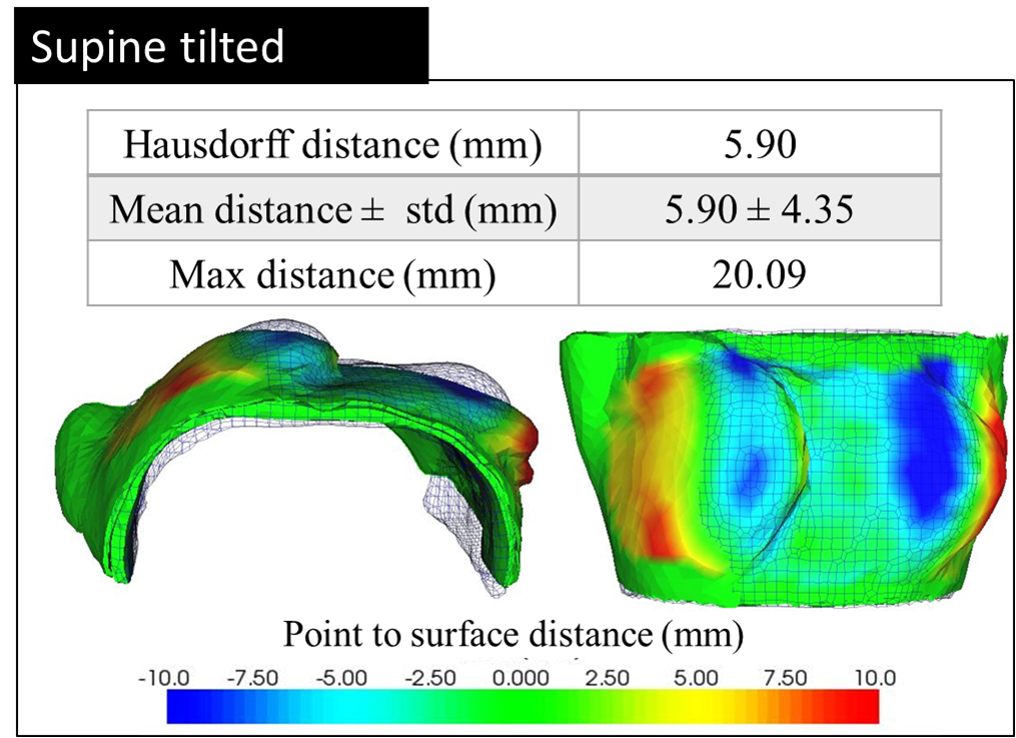
\includegraphics[width=0.6\textwidth,keepaspectratio]{figures/modelevaluation.png} 
\caption{Difference between estimated and measured breast geometries in supine tilted configuration.}\label{fig:modelevaluation}
\end{figure}

One may see that the supine tilted breast configuration is unwell described be the breast biomechanical model (Hausdorff distance equal to 5.90 mm). Large difference between simulated and measured breast surfaces is caused by the excessive sliding of breast tissues over the chest wall. Numerical or structural modeling choices could explain such a behavior.

Firstly, the fascial and ligamentous tissues are usually characterized by a cable-like behavior. The strain-energy density function must behave asymptotically in order to limit the fascia stretch and thus to reduce non-linearly the breast sliding over the chest wall. Limitations of the neo-Hookean model to capture the mechanical response of some nonlinear materials is well known \citep{kaliske_finite_1997}. For large strain rates, the Neo-Hookean material may undergo a relaxation and therefore becomes easier to deform.  Our numerical results have shown that the maximal strain at the fascia level is significantly higher in supine tilted position (about 140\%) than in supine or prone positions (about 50\%).  Therefore, an asymptotic behavior of fascia mechanical response must be considered.  The Gent  form of the strain-energy function characterizes better such mechanical response \citep{gent_new_1996} and will be considered as an alternative choice .

Secondly, the breast support matrix is composed of 4 suspensory ligaments, however only three of them were partially modeled: inframammary, deep medial and deep lateral ligaments. The 3D structures connecting the skin to some muscular areas, namely the cranial ligament,  were neglected.  The particularity  of the cranial ligament consists in its position. Indeed,  almost its entire structure underlies the skin and the only attachments to the thorax are situated at the clavicle and seventh rib levels (inframammary ligament). Including such structures at the skin surface may result in local high strain gradient rates causing solution instability and anesthetic surface deformations. 


\section{Discussions and conclusion} \label{section:validation:discutionconclusion}

In this chapter, a new finite element breast model was proposed and  evaluated with real tissues deformations measured on MR images. To this end, MR images of two volunteers were acquired in three different configurations: supine, prone and supine tilted. The supine and prone MRI volumes were used to adapt the biomechanical model to the volunteer individual breast geometry and its respective tissues mechanical properties.  The optimal mechanical properties were found by exhaustive search over a predefined parameters domain. For each combination of tissues elastic properties,  the breast reference configuration was computed using an adapted prediction-correction iterative scheme. The parameters set giving the best fit between estimated and measured breast configurations was selected.  Using these optimal estimates, the supine, prone and supine tilted breast configurations were computed and compared to the MRI volumes.

It was found that, extremely soft materials laws (0.2-0.3kPa for breast tissues and 4kPa for skin) have to by used in order to obtain the same tissues displacements rate as measured on MR images. Moreover, the breast tissues sliding have to be considered when computing such large deformations. However, because of tissues hyper-elasticity, the model boundary conditions have to be revisited in order to ensure the convergence capability of the solution. With such soft tissues, the finite element mesh may become highly distorted. Therefore to limit elements distortion a stiffer layer was added between the breast tissues and muscle representing the deep layer of the superficial fascia. The excessive  sliding was prevented by using ligamentous structures fixing the soft tissues on the pectoral muscle.

Contrary to the previous works, our model is evaluated in 3 breast configurations. Among the 3 geometries, two of them were used for the model optimization and evaluation, and the last one (supine tilted geometry) was used for the evaluation only. Good estimates were obtained in prone and supine configurations with a Hausdorff distance equal to $2.17 mm$ and $1.72 mm$ respectively.  The estimate of the supine tilted breast geometry pointed out the limitations of the Neo-Hookean model to assess rich mechanical behavior of breast soft tissues for large strains. These limitations were not identified in the previous works. 

The model optimization if a tough and time consuming process. It was extremely difficult to obtain the solutions convergence when combining the tissues large deformations with the sliding contact conditions. Because of the large computation time, the reference breast configuration and the optimal constitutive parameters were computed only for the first volunteer. The model optimization of the second volunteer is considered for future work.

Assuming that our model describes well the breast mechanical behavior, it can be used to compute breast tissues deformation under compression. In that case, internal tissues strains and the pressure distribution over the skin surface will be used to quantify the patient comfort during a mammography exam. 
   